\section{Implementation of LTC n-dimension}
\label{sec:implementation}
To implement \acrshort{ltc} in n dimensions with the infinity norm, we maintain a cuboid
representation of $\cap_{l=1}^j{\mathcal{B}_l}$ across the iterations of the
\texttt{while} loop in Algorithm~\ref{algo:general-ltc}. The implementation
works with constant memory and requires limited CPU time.

% With the Euclidean norm, the intersection test is more complex. We keep in
% memory a growing set $S$ of n-balls and the bounding box $B$ of their
% intersection. 
With the Euclidean norm, the intersection test is more complex. We keep in
memory a growing set $S$ of n-balls and the bounding box $B$ which represents an
approximate range of their intersection. We define $B$ as follows:
\begin{equation*}
    B = \bigcap_{l=1}^{j-1} box(\mathcal{B}_l) 
\end{equation*}
Where \texttt{box()} is a function that returns the bounding box of an n-ball.
Then, when a new point arrives, we consider the associated n-ball
$\mathcal{B}_j$ and our intersection test works as in
Algorithm~\ref{algo:euclidean}. Firstly, we check the intersection between
box($\mathcal{B}_j$) and $B$ (Algorithm~\ref{algo:euclidean}, line 11). To
restrict memory usage, $B$ only covers a set $S$ of n-balls were the size of $S$
is limited to $L_s$. Secondly, for each $\mathcal{B}_i$ in $S$, we check the
intersection between $\mathcal{B}_i$ and $\mathcal{B}_j$ (line 14). In addition
$\mathcal{B}_i$ will be removed if it includes $\mathcal{B}_j$, because if
$\mathcal{B}_j$ has intersection with n-balls in $S$ then a bigger n-ball which
contains $\mathcal{B}_j$ must also have intersection.
% \english{because smaller n-ball intersects
% $\mathcal{B}_j$ than a bigger n-ball which contains the smaller one (line 17, 18 in
% Algorithm~\ref{algo:euclidean})} \TG{English is not correct}.
Finally, we search a point in intersection of all n-balls in $S$, using plane
sweep~\cite{shamos1976geometric, souvaine2008line} and bisection initialized by
the bounds of $B$. Function \texttt{find\_bisection(S, B)} (see
Algorithm~\ref{algo:find_bisection_function}) and \texttt{recursive(S, L, R, N,
$X^n$)} (see Algorithm~\ref{algo:recursive}) show how it works. 

% describe function find_bisection
In function \texttt{find\_bisection(S, B)}, we selected dimension of n-balls as
$n$ used at the beginning of bisection, also computed minimum/maximum value of
bounding box $B$ at the $n_{th}$ dimension, which corresponds to $left$ and
$right$ in bisection method. The return object $X^n$ represents a n-dimensional
point in the intersection of all n-balls in $S$. It would be returned if we have
$True$ result from function \texttt{recursive(S, L, R, N, $X^n$)}. $X^n$ is
initialized and put into function \texttt{recursive(S, L, R, N, $X^n$)}, because
it is necessary to update the values (see Algorithm~\ref{algo:recursive} line
26) of $X^n$ during the recursive process. In line 27 of
Algorithm~\ref{algo:recursive}, it happens in case of $left > right$, which
means:
\begin{equation*}
    mid \  \bigcap \  (min\_id \cap max\_id) = \text{\O}
\end{equation*}

In Algorithm~\ref{algo:euclidean} line 14 and 15, it is guaranteed that any two
n-balls in $S$ has intersection. Therefore, any point in the intersection of
$min\_id$ and $max\_id$, could be used for determining the direction of
bisection. In our implementation, we select a point in connection of these two
n-ball's center, which also locates in intersecting object (line/chord when
order=2, plane/circle when order=3). Figure~\ref{fig:compare_point} shows the
point we selected in 2D.

%discuss the time complexity
According to our implementation for Euclidean norm, if the $L_s$ is undefined
($L_s$ is infinity), the operations in Algorithm~\ref{algo:euclidean} and
Algorithm~\ref{algo:find_bisection_function} before the function
\texttt{recursive()} need $O(n)$ complexity. In the \texttt{recursive()}
function, the bisection from line 12 to line 32 in
Algorithm~\ref{algo:recursive} needs $O(\log{2\epsilon})$, because the $left$
and $right$ are initialized from the bounding box $B$, where $|left - right|
\leqslant 2\epsilon$. Moreover, computing $left$ and $right$ which used for next
dimension in \texttt{recursive()} function needs $O(n)$. Thereby, when the data
stream is two-dimensional, the time complexity of LTC n-dimension for Euclidean
norm is $O(n) + O(\log{2\epsilon})\times O(n)$ = $O(n \times \log{2\epsilon})$,
where $n$ is the number of the data points we seen so far. In the same way, if
we process 3-dimensional stream with our algorithm with Euclidean norm, it needs
extra $O(n \times \log{2\epsilon})$ time in recursion, the total time complexity
is $O(n) + O(\log{2\epsilon})\times (O(n) + O(\log{2\epsilon})\times O(n))$ =
$O(n\times(\log{2\epsilon})^{2})$. Finally, our implementation for Euclidean
norm gives $O(n\times(\log{2\epsilon})^{d-1})$ time complexity for d-dimensional
data stream.


\begin{figure}
  \centering
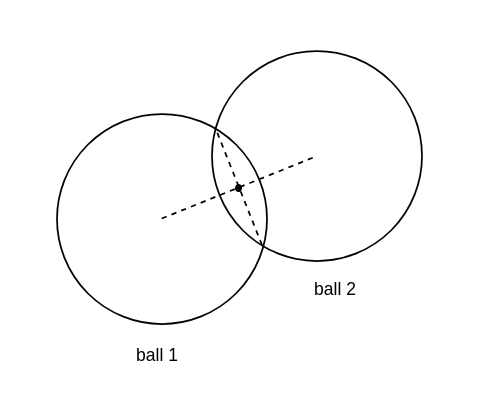
\includegraphics[width=0.7\textwidth]{figures/point-in-chord.png}
\caption{The point selected to determine the direction}
\label{fig:compare_point}
\end{figure}


\begin{algorithm}
\begin{algorithmic}[1]
\Input
    \Desc{$S$}{Set of intersecting n-balls}
    \Desc{$B$}{Bounding box of the intersection of n-balls in $S$}
    \Desc{$\mathcal{B}_j$}{New n-ball to check}
    \Desc{$L_s$}{The maximum length of $S$}
\EndInput
\Output
    \Desc{$S$}{Updated set of intersecting n-balls}
    \Desc{$B$}{Updated bounding box}
    \Desc{$T$}{True if all the n-balls in S and $\mathcal{B}_j$ intersect}
    \Desc{$x$}{Point inside intersection. It might be Null}
\EndOutput

%\If{$\mathcal{B}_j \cap B = \text{\O}$} \Comment{Ball is outside bounding box}
\If{$S$.length $\geqslant L_s \parallel$ box($\mathcal{B}_j$) $\cap B = \text{\O}$} \Comment{N-ball is outside bounding box}
    \State \Return ($S$, $B$, False, Null)
\EndIf
\If{$\exists\ \mathcal{B}_i \in S$ s.t. $\mathcal{B}_j \cap \mathcal{B}_i = \text{\O}$}
    \State \Return ($S$, $B$, False, Null) \Comment{Some n-balls don't intersect}
\EndIf
\If{$\exists\ \mathcal{B}_i \in S$ s.t. $\mathcal{B}_j \subset \mathcal{B}_i$} \Comment{Remove inclusions}
%\State Remove $\mathcal{B}_i$ from $B$. %Add $\mathcal{B}_j$ to $B$. 
    \State Remove $\mathcal{B}_i$ from $S$. %Add $\mathcal{B}_j$ to $S$. 
\EndIf
\State $B$ = box($\mathcal{B}_j$) $\ \bigcap\ $ $B$
\State $S$ = $S \ \bigcup \  \{\mathcal{B}_j\}$
\State $x$ = find\_bisection($S$, $B$) \Comment{This can take some time}
\If{$x$ == Null}
    \State \Return ($S$, $B$, False, Null)
\Else
    \State \Return ($S$, $B$, True, $x$)
\EndIf
\end{algorithmic}
\caption{Intersection test for Euclidean n-balls.}
\label{algo:euclidean}
\end{algorithm}


\begin{algorithm}[H]
\begin{algorithmic}[1]
\Input
    \Desc{$S$}{Set of n-balls}
    \Desc{$B$}{Bounding box of the intersection of n-balls in $S$}
\EndInput
\Output
    \Desc{$X^n$}{N-dimensional point in all n-balls in $S$, $X^n = (x_1,...,x_n)$}
\EndOutput

\State $n$ = dimension of n-balls
\State $left$ = min\_value($B$, $n$) \Comment{Minimum value of $B$ along $n^{th}$ dimension}
\State $right$ = max\_value($B$, $n$) \Comment{Maximum value of $B$ along $n^{th}$ dimension}
\State $X^n$ = Null
\If{recursive(S, left, right, n, $X^n$)}
    \State \Return $X^n$
\Else
    \State \Return Null
\EndIf
\end{algorithmic}
\caption{Function find\_bisection(S, B)}
\label{algo:find_bisection_function}
\end{algorithm}

\begin{algorithm}
\begin{algorithmic}[1]
\Input
   \Desc{$S$}{Set of n-balls}
   \Desc{$L$}{Min value used in bisection}
   \Desc{$R$}{Max value used in bisection}
   \Desc{$N$}{The $N^{th}$ dimension, $N \in \{1...n\}$}
   \Desc{$X^n$}{N-dimensional point which records point of intersection, $X^n$ = $(x_1,...,x_n)$} 
   %\TG{\#\#If you know the point already, what are you looking for?}
\EndInput
\Output
   \Desc{$T$}{True if a point is found by using bisection}
\EndOutput
\If{$N$ == 1}
    \State $X^n.x_N$ = $\frac{L+R}{2}$; $\ $\Return True
\EndIf
\While{$L < R$ }
    \State $mid$ = $\frac{L+R}{2}$; $\ surface$ = $\{x_{N}...x_{n}\}$
    \State $left$ = -$\infty$; $\ right$ = +$\infty$
    \ForAll{$\mathcal{B}_i \in S$}
        \State $min$ = min\_value($\mathcal{B}_i \cap surface$, N-1)
        \State $max$ = max\_value($\mathcal{B}_i \cap surface$, N-1)
        \If{$left < min$}
            \State $left$ = $min$; $\ min\_id$ = $\mathcal{B}_i$
        \EndIf
        \If{$right > max$}
            \State $right$ = $max$; $\ max\_id$ = $\mathcal{B}_i$
        \EndIf
    \EndFor
    
    \If{$left \leqslant right$}
        \State $X^n.x_N$ = $mid$; $\ $
        \Return recursive($S$, $left$, $right$, $N-1$, $X^n$)
    \ElsIf{$\ \forall\ P$ (Point) $\in (min\_id \cap max\_id)$ s.t. $P.x_N < mid$}
        \State $R$ = $mid$
    \Else
        \State $L$ = $mid$
    \EndIf
\EndWhile
\State \Return False
\end{algorithmic}
\caption{Function recursive(S, L, R, N, $X^n$)}
\label{algo:recursive}
\end{algorithm}
